% !TEX encoding = UTF-8 Unicode
% !TEX root =  ../Bachelorarbeit.tex

\chapter{Hauptteil}
\label{cha:Hauptteil}

\section{\"uberblick \"uber die Entwicklungsplattform MSP430FR5729}
\label{EntwicklungsplattformMSP430FR5729}

Die Auswahl einer geeigneten Entwicklungsplattform bildet die Grundlage f\"ur die erfolgreiche Implementierung und Evaluierung eingebetteter Systeme. Im Rahmen dieser Arbeit dient der MSP430FR5729 von Texas Instruments als zentrale Hardwarekomponente. Dessen Architektur und Funktionalit\"aten werden in den folgenden Abschnitten n\"aher betrachtet.

Der MSP430FR5729 ist ein Low-Power-Microcontroller  \Fachbegriff[Mikrocontroller mit 16-Bit-Registerbreite und reduzierter Befehlssatzarchitektur (Reduced Instruction Set Computer)]{16-Bit-RISC-Microcontroller} von Texas Instruments mit einer Maximalen Taktfrequenz von Acht \Fachbegriff[Ma{\ss}einheit für die Frequenz und entspricht einer Million Schwingungen pro Sekunde (1 MHz = 10$^{6}$ Rechenschritte).]{Megaherz}. Eingebaute Low-Power-Modi (\Abkuerzung{Low Power Mod}{LPM}s), (Auflistung aller Modi in \Abbildung{operation_modes}) erm\"oglichen \ua niedrigere Taktfrequenzen und das deaktivieren von Oszillatoren, wodurch er sich besonders gut f\"ur energieeffiziente Anwendungen im Bereich eingebetteter Systeme eignet. \Zitat[S. 43, Kap. 6.3, S. 35, Kap. 1.4 \& S. 37, Kp. 1.4.1]{ti:slase35c, ti:slau272d}

\begin{figure}[h!]
	\centering
	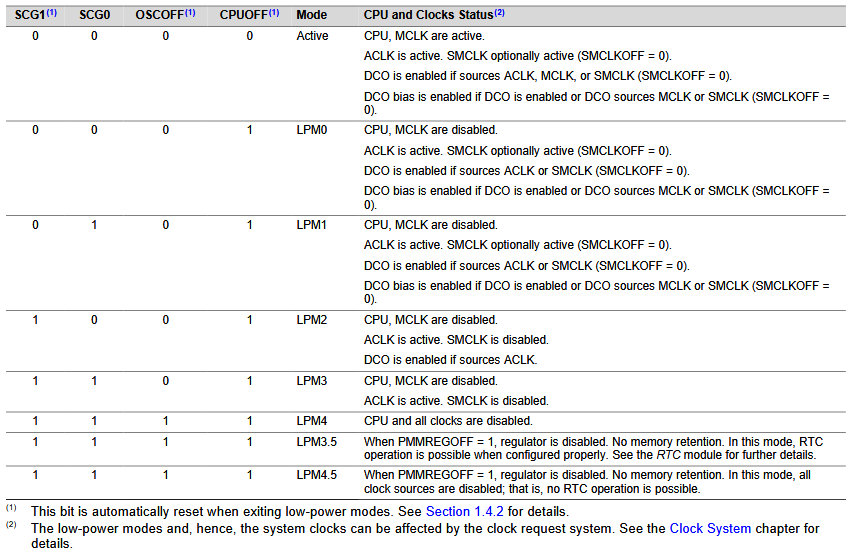
\includegraphics[width=1.0\textwidth]{../Bilder/Operating_Modes.png}
	\caption{Operating Modes\\\Zitat[S. 37, Kap. 1.4, Tab. 1-2]{ti:slau272d}}
	\label{fig:operation_modes}
\end{figure}

Der Mikroprozessor besitzt 16 Kilobyte an nicht-fl\"uchtigen FRAM, sowie ein Kilobyte \Fachbegriff[Schnellster, fl\"uchtiger Speicher mit geringer Kapazit\"at, bestehend aus Flip-Flops welcher meist direkt in der CPU mit eingebaut ist.]{statischen Arbeitsspeicher} (\Abkuerzung{Static Random Access Memory}{SRAM}). 

Die Versorgungsspannung betr\"agt 2 bis 3,6 Volt wobei ebenfalls verschiedene Low-Power-Modi verwendet werden k\"onnen, um den Stromverbrauch zunehmend zu minimieren. Diese beeinflussen den sp\"ateren Umgang mit Timer-Interrupts, weil sie den Energieverbrauch im Wartezustand beeinflussen. \Zitat[S. 26, Kap. 5.20]{ti:slase35c}

Des Weiteren besitzt der Chip F\"unf Interne 16-Bit Timer mit jeweils Sieben\\\NeuerBegriff{Capture and Compare} Registerbl\"ocken. Diese internen Timer stellen eine zentrale Komponente f\"ur die Realisierung pr\"aziser Zeitgesteuerter Funktionen und die Generierung von Interrupts dar, welche im nachfolgenden Kapitel \ref{TIMER&ISR} tiefgreifender erl\"autert werden.

Zur externen Kommunikation sind Protokolle wie \Abkuerzung{Universal Asynchronous Receiver Transmitter}{UART}, \Abkuerzung{Inter-Integrated Circuit}{I$^{2}$C} und \Abkuerzung{Serial Peripheral Interface}{SPI} integriert, welche mit 32 Programmierbaren \Abkuerzung{General Purpose Input/Output}{GPIO}-Pins angeschlossen werden k\"onnen. Kommunikationsschnittstellen sind f\"ur die Interaktion mit der Au{\ss}enwelt und Peripherieger\"aten von hoher Bedeutung. Eine detailliertere Ausarbeitung des \Fachbegriff[Serielle Schnittstelle in Mikrocontrollern von Texas Instruments, die verschiedene Kommunikationsprotokolle (\zB UART, SPI, I$^{2}$C) unterst\"utzt.]{enhanced Universal Serial Communication Interface} (\Abkuerzung{enhanced Universal Serial Communication Interface}{eUSCI}) in Kapitel \ref{eUSCI}. \Zitat[S. 1, Kap. 1.1]{ti:slase35c}

\begin{figure}[h!]
	\centering
	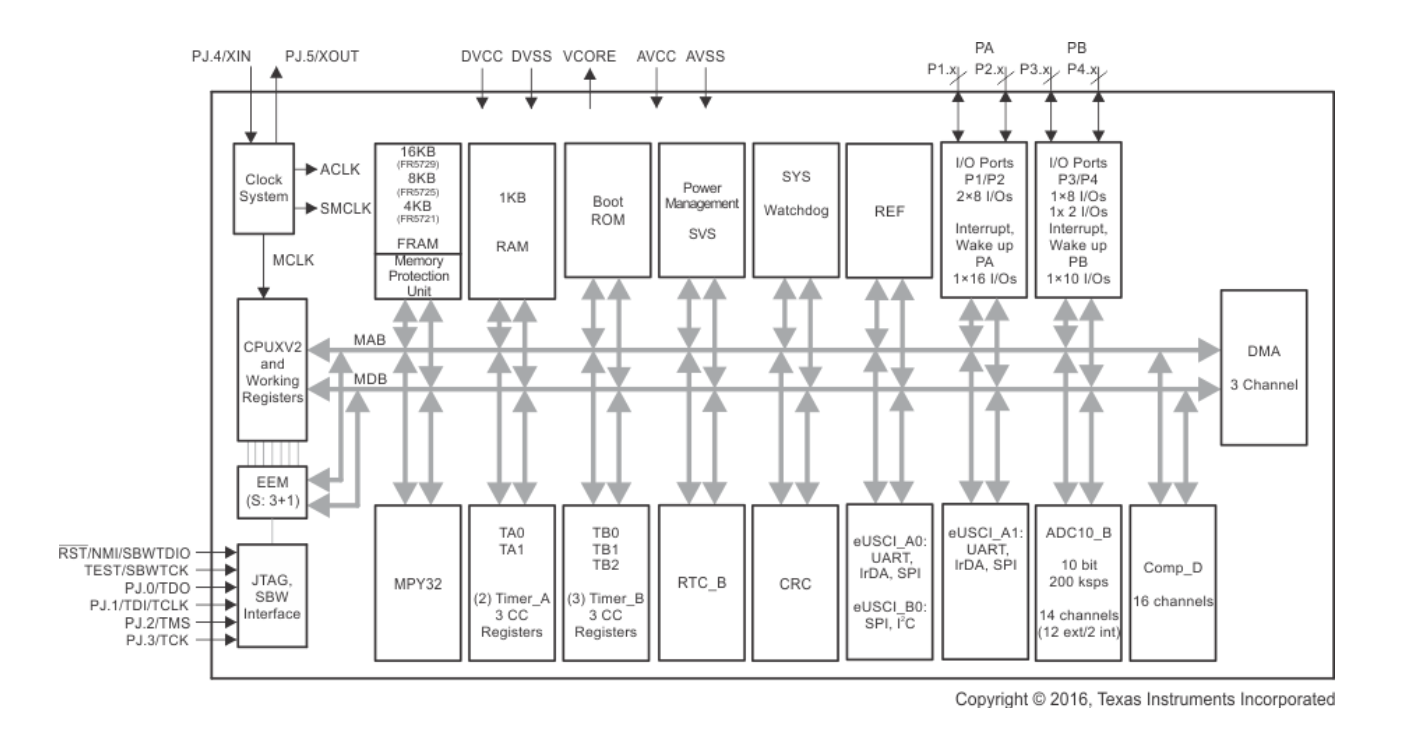
\includegraphics[width=1.0\textwidth]{../Bilder/FunctionalBlockDiagram_MSP430FR5729.png}
	\caption{Block Diagramm MSP430FR5729\\Mikrocontroller \Zitat[S. 2, Kap. 1.4]{ti:slase35c}}
	\label{fig:BlockDiagramm_msp430}
\end{figure}

\newpage
\Abbildung{BlockDiagramm_msp430} zeigt ein vollst\"andiges Block Diagramm des Mikroprozessors, welches noch einige weitere Eigenschaften, Funktionen und Subsysteme auflistet. \AI


\subsection{Timer und Interrupt Service Routinen (ISR)}
\label{TIMER&ISR}

Timer und Interrupt Service Routinen (\Abkuerzung{Interrupt Service Routine}{ISR}s) stellen einen fundamentalen Baustein moderner eingebetteter Systeme dar. Sie erm\"oglichen pr\"azise, zeitgesteuerte Funktionen als auch das reagieren auf externe Ereignisse. Womit die Realisierungen komplexer, Echtzeitsysteme m\"oglich wird. Im Folgenden wird die Timer-Architektur des MSP430FR5729 und die zugeh\"origen ISR-Mechanismen detailliert betrachtet.

Der MSP430FR5729 verf\"ugt \"uber insgesamt f\"unf 16-Bit-Timer, wobei zwei dem Typ A und drei dem Typ B angeh\"oren. Beide Typen erm\"oglichen vielseitige Zeitsteuerungsfunktionen, weisen jedoch spezifische Unterschiede in ihren Konfigurationsm\"oglichkeiten auf.

Beide Timer-Typen verf\"ugen \"uber einen gemeinsamen 16-Bit-Z\"ahler sowie sieben Capture/Compare-Register. Diese Register erm\"oglichen die Implementierung verschiedenster Funktionen. Die Capture-Funktionalit\"at dient dazu, den aktuellen Z\"ahlerwert bei einem externen oder internen Ereignis pr\"azise zu erfassen. Dies ist beispielsweise n\"utzlich f\"ur die Messung von Pulsweiten oder Frequenzen. Die Compare-Funktionalit\"at hingegen erlaubt den Vergleich des aktuellen Z\"ahlerstandes mit einem in den Compare-Registern hinterlegten Wert. Bei einer \"ubereinstimmung kann eine konfigurierbare Aktion ausgel\"ost werden, wie beispielsweise das Setzen oder R\"ucksetzen eines Ausgangspins oder das Generieren eines Interrupts. Die vielseitigen Einstellungsm\"oglichkeiten dieser Register erlauben die Realisierung komplexer Zeitgesteuerter Aufgaben. \Zitat[S. 333, Kap. 11 \& S. 355, Kap. 12, S. 287, Kap. 8.3 \& S. 194, Kap. 6.8.2]{ti:slau272d,davies:msp430}

Die Timer des Typs B weisen im Vergleich zu dem Timer des Typs A, erweiterte Konfigurationsm\"oglichkeiten auf. Darunter fällt die Konfigurierbarkeit der Timer-L\"ange auf 8, 10, 12 oder 16 Bit, was eine flexible Anpassung der Z\"ahlaufl\"osung und der \"uberlaufperiode f\"ur unterschiedliche Aufl\"osungen erm\"oglicht. Weiterhin sind alle Capture/Compare-Bl\"ocke doppelt gepuffert. Diese doppelte Pufferung erlaubt das Laden neuer Vergleichswerte, w\"ahrend eines aktiven Z\"ahlzyklus, wodurch unerw\"unschte Effekte oder Inkonsistenzen in den Ausgangssignalen vermieden werden. Zudem k\"onnen alle Ausg\"ange auf einen hochohmigen Zustand umgeschaltet werden, was in bestimmten Applikationen vorteilhaft sein kann. Ein weiterer wichtiger Unterschied besteht darin, dass die Capture/Compare-Eing\"ange nicht synchronisiert sind und somit asynchron zu dem internen Takt des Timers operieren k\"onnen, was in bestimmten Szenarien die Erfassung externer Ereignisse erleichtert. \Zitat[S. 356, Kap. 12.1.1, S. 353, Kap. 8.9]{ti:slau272d, davies:msp430}

F\"ur die pr\"azise Steuerung und Ereignisbehandlung bieten die Timer verschiedene Betriebsarten, die im Folgenden n\"aher erl\"autert werden.

\newpage
\subsubsection{Timer Zählweisen}
\label{Timer_CountMode}

Der Z\"ahlmodus, bestimmt die interne Z\"ahlweise des Timers. Die Timer unterst\"utzen typischerweise mehrere Varianten dieses Modus, um unterschiedlichen Anforderungen gerecht zu werden. \Zitat[S. 291, Kap. 8.3.1]{davies:msp430}

\begin{itemize}
	\item \textbf{Up Mode:} Im Up Mode (Additive Z\"ahlweise) beginnt der Z\"ahler bei Null und inkrementiert seinen Wert mit jedem Taktimpuls der gew\"ahlten \Fachbegriff[Eine Referenz auf ein periodisches Zeitsignal um zeitliche Abl\"aufe zu synchronisieren; typischerweise in Form von Quarzoszillatoren oder externen Taktsignalen.]{Clock-Source}. Er erreicht einen vordefinierten Maximalwert, der im Compare-Register gespeichert ist, und beginnt dann wieder von Null zu z\"ahlen. Ein \"uberlauf-Interrupt wird generiert, sobald der Z\"ahler den Wert von CCR0 erreicht. Dieser Modus eignet sich ideal f\"ur die Erzeugung periodischer Ereignisse oder die Messung von Zeitintervallen bis zu einem bestimmten Grenzwert. Beispielsweise kann durch die Wahl einer geeigneten Clock-Source und eines passenden Wertes im Compare-Register eine pr\"azise Zeitbasis f\"ur periodische Aufgaben geschaffen werden. \Zitat[S. 337, Kap. 11.2.3.1 \& S. 359, Kap. 12.2.3.1, S. 330, Kap. 8.6]{ti:slau272d, davies:msp430}
	
	\item \textbf{Continuous Mode:} Der Continuous Mode l\"asst den Z\"ahler von Null bis zum maximal m\"oglichen Wert (FFFFh f\"ur 16-Bit-Timer) z\"ahlen und anschlie{\ss}end wieder bei Null beginnen. Ein \"uberlauf-Interrupt wird generiert, wenn der Z\"ahler vom Wert von FFFFh auf 0 \"uberl\"auft. \Zitat[S. 338, Kap. 11.2.3.2 \& S. 360, Kap. 12.2.3.2]{ti:slau272d} Dieser Modus ist besonders n\"utzlich, wenn l\"angere, voneinander unabh\"angige Zeitintervalle zu messen oder wenn eine freilaufende Zeitbasis ben\"otigt wird, um Ereignisse in Bezug auf den Z\"ahlerstand, ohne einen periodischen Neustart durch das Compare-Register, zu erfassen. \Zitat[S. 338, Kap. 11.2.3.3 \& S. 360, Kap. 12.2.3.3, S. 318, Kap. 8.5]{ti:slau272d, davies:msp430}

	\item \textbf{Up/Down Mode:} Der Up/Down Mode (Auf-/Abw\"artsz\"ahlmodus) kombiniert das Auf- und Abz\"ahlen. Der Z\"ahler beginnt bei Null, z\"ahlt Zyklisch bis zum festgelegten Wert im Compare-Register und dann wieder bis Null herunter. Ein \"uberlauf-Interrupt wird generiert, wenn der Z\"ahler den Wert von CCR0 erreicht, und ein weiterer Interrupt (sofern aktiviert) kann beim Erreichen von Null gesetzt werden. \Zitat[S. 339, Kap. 11.2.3.4 \& S. 361, Kap. 12.2.3.4]{ti:slau272d} Dieser Modus erzeugt eine symmetrische \Fachbegriff[Ein Verfahren zur Steuerung der Leistungszufuhr, bei dem die mittlere Ausgangsleistung durch Variieren des Abtastverh\"altnisses eines Rechtecksignals reguliert wird.]{Pulsweitenmodulation (PWM)} und wird h\"aufig in Anwendungen zur Motorsteuerung oder zur Erzeugung pr\"aziser analoger Ausgangssignale eingesetzt. \Zitat[S. 340, Kap. 11.2.3.5 \& S. 362, Kap. 12.2.3.5, S. 349, Kap. 8.7]{ti:slau272d, davies:msp430}
\end{itemize}

Die Wahl eines geeigneten Modus h\"angt stark von der spezifischen Anwendung ab. F\"ur einfache Zeitmessungen oder periodische Aufgaben ist der Up Mode oft ausreichend, w\"ahrend der Continuous Mode f\"ur l\"angere Intervalle oder als Basis f\"ur komplexere Zeitsteuerungen dient. Der Up/Down Mode hingegen findet seine Anwendung prim\"ar in der Erzeugung von Steuersignalen.

\subsubsection{Capture-Mode}
\label{Timer_CaptureMode}

Der Capture Mode erm\"oglicht es, den aktuellen Wert des Z\"ahlers pr\"azise zu erfassen, wenn ein bestimmtes Ereignis an einem zugeh\"origen Eingangspin auftritt. Der erfasste Z\"ahlerwert wird in einem der Capture-Register (CCR0 bis CCR6) gespeichert. Dies ist besonders n\"utzlich f\"ur die Messung von externen Signalen wie Pulsweiten, Frequenzen oder der Zeit zwischen zwei Ereignissen. Beispiele hierzu in \Abbildung{CaptureModeBeispiele}.

\begin{figure}[h!]
	\centering
	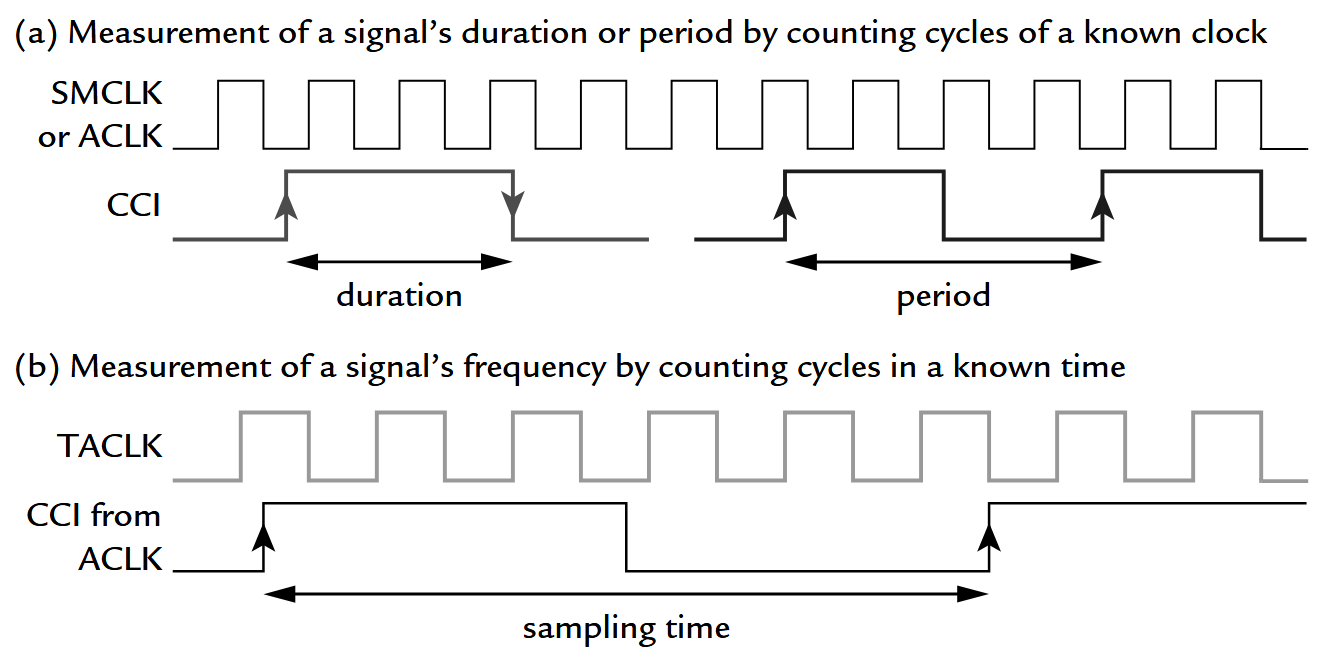
\includegraphics[width=1.0\textwidth]{../Bilder/CaptureMode_Beispiele.png}
	\caption{Capture Mode Einsatzbeispiele\\\Zitat[S. 301, Abb. 8.7]{davies:msp430}}
	\label{fig:CaptureModeBeispiele}
\end{figure}

Die Timer des MSP430FR5729 unterst\"utzen verschiedene Capture-Modi. Diese legen fest, bei welcher Art von Signal\"anderung die Erfassung des Z\"ahlerwertes erfolgt:

\begin{itemize}
	\item \textbf{Capture on rising edge:} Sobald am zugeh\"origen Eingangspin eine steigende Flanke detektiert wird (\"ubergang von Low nach High) wird in diesem Modus der aktuelle Z\"ahlerwert in das Capture-Register geschrieben.

	\item \textbf{Capture on falling edge:} Hier erfolgt die Erfassung des Z\"ahlerwertes am Eingangspin bei einer fallenden Flanke (\"ubergang von High nach Low).

	\item \textbf{Capture on both edges:} Dieser Modus erm\"oglicht die Erfassung des Z\"ahlerwertes sowohl bei steigender als auch fallender Flanken. Dies ist besonders praktisch f\"ur die Messung von Signalperioden oder bei Relevanz beider Flanken eines Signals.
\end{itemize}

Sofern ein Interrupt im entsprechenden Capture-Register aktiviert ist, kann dieser auch Interrupts ausl\"osen. In der zugeh\"origen ISR kann der erfasste Z\"ahlerwert aus dem Capture-Register gelesen und weiterverarbeitet werden. Mehrere Capture-Register innerhalb eines Timers erm\"oglichen die Erfassung und Auswertung mehrerer aufeinanderfolgender Ereignisse, ohne dass der vorherige Wert \"uberschrieben wird. 

Die Konfiguration des Capture Mode umfasst die Auswahl des ausl\"osenden Ereignisses (Flanke) sowie \ggf die Aktivierung des Capture-Interrupts. Die erfassten Zeitstempel im Capture-Register erlauben pr\"azise Messungen und die Analyse externer Signale in eingebetteten Systemen. \Zitat[S. 340, Kap. 11.2.4.1 \& S. 362, Kap. 12.2.4.1, S. 300, Kap. 8.4]{ti:slau272d, davies:msp430}

\subsubsection{Compare-Mode}
\label{Timer_CompareMode}

Der Compare Mode erm\"oglicht es, den aktuellen Wert des Z\"ahlers kontinuierlich mit den in den Compare-Registern CCR0 bis CCR7 hinterlegten Werten zu vergleichen. Wenn der Z\"ahlerstand mit dem Vergleichswert \"ubereinstimmt, kann \zB ein Interrupt ausgel\"ost oder ein Ausgangspin beeinflusst werden.

Die Compare-Modi bieten verschiedene M\"oglichkeiten, wie der Ausgangspin bei einer \"ubereinstimmung beeinflusst werden soll:

\begin{itemize}
	\item \textbf{Set output on compare:} Bei einer \"ubereinstimmung des Z\"ahlerstandes mit dem Compare-Registerwert wird der zugeh\"orige Ausgangspin auf High gesetzt.

	\item \textbf{Reset output on compare:} Hier wird der Ausgangspin bei \"ubereinstimmung auf Low gesetzt.

	\item \textbf{Toggle output on compare:} In diesem Modus \"andert der Ausgangspin bei jeder \"ubereinstimmung seinen Zustand (von High nach Low oder von Low nach High).

	\item \textbf{Output High:} Der Ausgangspin wird permanent auf High gehalten.

	\item \textbf{Output Low:} Der Ausgangspin wird permanent auf Low gehalten.

	\item \textbf{Set/Reset:} In Kombination mit dem Compare-Register 0 (CCR0) kann ein PWM-Signal erzeugt werden. Beispielsweise kann der Ausgang bei Erreichen des CCR0-Wertes gesetzt und bei Erreichen des CCRn-Wertes zur\"uckgesetzt werden (oder umgekehrt), wobei CCRn die Pulsweite bestimmt.
\end{itemize}

\Abbildung{OutputUnit_UpDown_Mode} zeigt eine m\"ogliche Konfiguration im Z\"ahlmodus Up/Down mit zwei Compare-Registern (TAxCCR1 \& TAxCCR2), eingestellt auf Toggle/Set und Toggle/Reset.

\begin{figure}[h!]
	\centering
	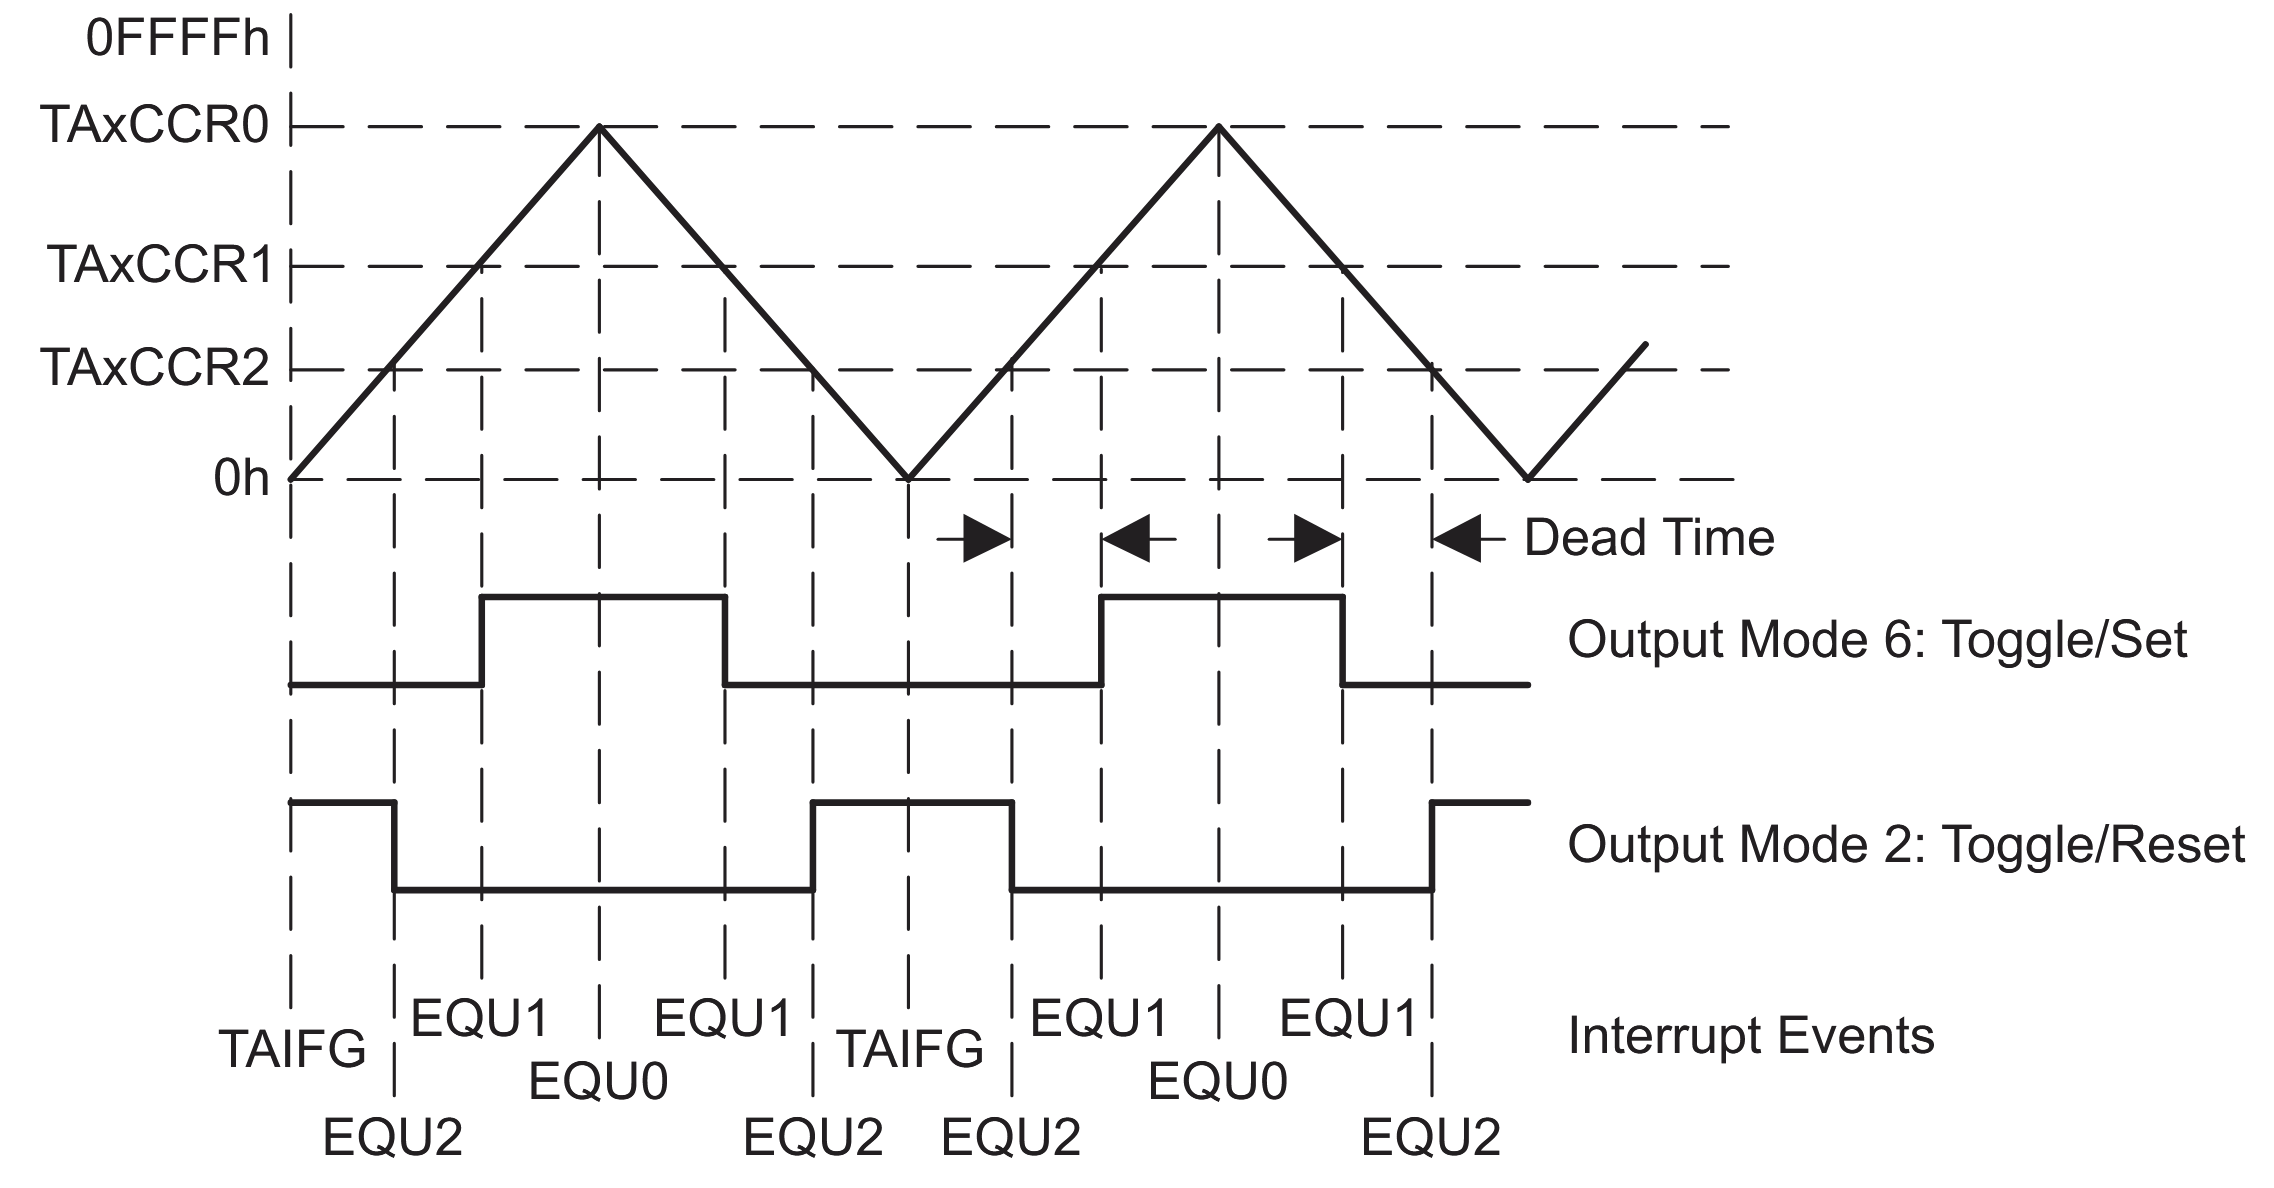
\includegraphics[width=1.0\textwidth]{../Bilder/UpDown_ModeBsp.png}
	\caption{Ausgabeeinheit im Up/Down-Modus\\\Zitat[S. 340, Abb. 11-9]{ti:slau272d}}
	\label{fig:OutputUnit_UpDown_Mode}
\end{figure}

\"Ahnlich wie beim Capture Mode erm\"oglicht ein Interrupt der CPU, auf pr\"azise Zeitpunkte zu reagieren und entsprechende Aktionen auszuf\"uhren. Der Compare Mode ist somit ein vielseitiges Werkzeug zur Erzeugung von Steuersignalen, zur Implementierung von Zeitverz\"ogerungen oder zur Synchronisation interner Operationen mit einer pr\"azisen Zeitbasis. \Zitat[S. 342, Kap. 11.2.4.2 \& S. 364, Kap. 12.2.4.2, S. 352, Kap. 8.8]{ti:slau272d, davies:msp430}

Nachdem die verschiedenen Betriebsarten des Timers betrachtet wurden, ist es wichtig zu verstehen, wie die zugeh\"origen Register konfiguriert werden, um die gew\"unschte Funktionalit\"at zu erzielen.


\subsubsection{Einstellungen der Capture and Compare Register}
\label{CC_Register}

Die Funktionalit\"at der Capture- und Compare-Einheiten wird ma{\ss}geblich durch die Konfiguration ihrer zugeh\"origen Register bestimmt. Hierzu geh\"oren die Aktivierung und Deaktivierung von Interrupts, die Auswahl des Ausgangsmodus (nur f\"ur Compare) sowie die Festlegung des ausl\"osenden Ereignisses.

F\"ur jedes Capture/Compare-Register kann individuell festgelegt werden, ob ein Interrupt ausgel\"ost werden soll, wenn ein entsprechendes Ereignis eintritt. Dies geschieht \"uber spezifische \NeuerBegriff{Interrupt-Enable-Bits} im jeweiligen Capture/Compare-Control-Register (TAxCCTLn oder TBxCCTLn). Durch das Setzen des CCIE-Bits auf Eins oder Null, kann die Generierung eines Interrupts bei einem Capture- oder Compare-Ereignis aktiviert \bzw deaktiviert werden. \Tabelle{tb_ccc_register} fasst alle weiteren Register des Timers B mit ihren Beschreibungen zusammen.


\begin{table}[h!]
	\small
	\centering
	\begin{tabular}{|c|l|c|c|p{8cm}|}
		\hline
		\textbf{Bit} & \textbf{Field} & \textbf{Type} & \textbf{Reset} & \textbf{Description} \\ \hline
		15-14 & CM & RW & 0h & Capture mode \\ \hline
		13-12 & CCIS & RW & 0h & Capture/compare input select. These bits select the TBxCCRn input signal. \\ \hline
		11 & SCS & RW & 0h & Synchronize capture source. This bit is used to synchronize the capture input signal with the timer clock. \\ \hline
		10-9 & CLLD & RW & 0h & Compare latch load. These bits select the compare latch load event.  \\ \hline
		8 & CAP & RW & 0h & Capture-/Compare mode \\ \hline
		7-5 & OUTMOD & RW & 0h & Output mode. \\ \hline
		4 & CCIE & RW & 0h & Capture/compare interrupt enable. This bit enables the interrupt request of the corresponding CCIFG flag. \\ \hline
		3 & CCI & R & Undef & Capture/compare input. The selected input signal can be read by this bit. \\ \hline
		2 & OUT & RW & 0h & Output. For output mode 0, this bit directly controls the state of the output. \\ \hline
		1 & COV & RW & 0h & Capture overflow. This bit indicates a capture overflow occurred. COV must be reset with software.  \\ \hline
		0 & CCIFG & RW & 0h & Capture/compare interrupt flag \\ \hline
	\end{tabular}
	\caption{Registerbeschreibung – Capture-/Compare Register Timer B\\\Zitat[S. 375, Tab. 12-8]{ti:slau272d}}
	\label{tab:tb_ccc_register}
\end{table}



Wie bereits im Abschnitt \ref{Timer_CompareMode} zum Compare Mode beschrieben, legen die Output Mode Bits (OUTMOD) fest, wie der zugeh\"orige Ausgangspin bei einer \"ubereinstimmung des Z\"ahlerstandes mit dem Compare-Registerwert beeinflusst wird. Die Auswahl des passenden Output Mode ist entscheidend f\"ur die Erzeugung der gew\"unschten Ausgangssignale, wie beispielsweise bei der Pulsweitenmodulation.

Die Auswahl des ausl\"osenden Ereignisses f\"ur eine Capture- oder Compare-Operation wird ebenfalls \"uber Bits im TAxCCTLn- oder TBxCCTLn-Register gesteuert. F\"ur den Capture Mode wird hier beispielsweise mit dem CM-Bit festgelegt, ob die Erfassung bei einer steigenden, fallenden oder beiden Flanken des Eingangssignals erfolgen soll. Im Compare Mode definiert diese Einstellung, unter welchen Bedingungen die Vergleichsoperation als erfolgreich betrachtet wird und die entsprechende Aktion (Interrupt, Ausgangssignal\"anderung) ausgel\"ost wird. Dies kann beispielsweise ein reiner Vergleich oder auch ein Vergleich in Kombination mit dem \"uberlauf des Z\"ahlers im Up Mode sein. \Zitat[S. 351, Kap. 11.3.3 \& S. 375, Kap. 12.3.3, S. 292, Kap. 8.3.2]{ti:slau272d, davies:msp430}

Die sorgf\"altige Konfiguration dieser Einstellungen in den Capture/Compare-Registern ist unerl\"asslich, um den Timer pr\"azise an die Anforderungen der jeweiligen Applikation anzupassen.

Ein weiterer fundamentaler Aspekt der Timer-Konfiguration ist \ua die Wahl der Taktquelle, welche die Zeitbasis f\"ur den Z\"ahler und somit f\"ur alle zeitgesteuerten Operationen des Timers bestimmt. \AI

\newpage
\subsubsection{Timer Control-Register}
\label{TimerControlRegister}

Die Timer des MSP430FR5729 k\"onnen von verschiedenen internen Taktquellen getaktet werden, die jeweils unterschiedliche Eigenschaften und Anwendungsbereiche aufweisen. Die prim\"aren Taktquellen sind \Fachbegriff[Niederfrequente Taktquelle in Mikrocontroller-Systemen, die typischerweise von einem Quarzoszillator gespeist wird und f\"ur energiesparende Betriebsmodi verwendet wird.]{Auxiliary Clock (ACLK)} und \Fachbegriff[Taktgesteuertes Signal, das typischerweise f\"ur Peripherieger\"ate verwendet wird und sich aus einer frei w\"ahlbaren Taktquelle ableiten l\"asst.]{Sub-Main Clock (SMCLK)}. Auch externe Taktquellen k\"onnen zur Taktung des Timers herangezogen werden wie \zB das TACLK/TBCLK-Register oder der INCLK-Pin. \Zitat[S. 71, Kap. 3.1, S. 163, Kap. 5.8 \& S. 289, Kap. 8.3.1]{ti:slau272d, davies:msp430}

Die Auswahl der Clock-Source f\"ur einen Timer erfolgt \"uber spezifische Bits im TAxCTL oder TBxCTL Timer Control Register. Das TASSEL-/TBSSEL-Bit legt fest, ob der Timer von TAxCLK/TBxCLK, ACLK, SMCLK oder INCLK getaktet wird. Die Wahl der Clock-Source hat einen direkten Einfluss auf die Timer-Frequenz, wobei die Timer-Frequenz nicht gleich der Frequenz der gew\"ahlten Clock-Source entsprechen muss. Durch optionale Prescaler-Werte wie dem ID-Bit und dem TAIDEX-/TBIDEX-Bit kann die Frequenz weiter individualisiert werden. \Zitat[S. 349, Kap. 11.3.1 \& S. 372, Kap. 12.3.1, S. 289, Kap. 8.3.1]{ti:slau272d, davies:msp430}

\begin{table}[h!]
	\small
	\centering
	\begin{tabular}{|c|l|c|c|p{8cm}|}
		\hline
		\textbf{Bit} & \textbf{Field} & \textbf{Type} & \textbf{Reset} & \textbf{Description} \\ \hline
		15 & Reserved & R & 0h & Reserved. Always reads as 0. \\ \hline
		14–13 & TBCLGRP & RW & 0h & \textbf{TBxCLn group:} Synchronously updates multiple Capture/Compare registers as needed. \\ \hline
		12–11 & CNTL & RW & 0h & Counter length \\ \hline
		10 & Reserved & R & 0h & Reserved. Always reads as 0. \\ \hline
		9–8 & TBSSEL & RW & 0h & clock source select \\ \hline
		7–6 & ID & RW & 0h & \textbf{Input divider:} together with TBIDEX divides the input clock \\ \hline
		5–4 & MC & RW & 0h & \textbf{Mode control:} \ref{Timer_CountMode} \\ \hline
		3 & Reserved & R & 0h & Reserved. Always reads as 0. \\ \hline
		2 & TBCLR & RW & 0h & Clears TBR and control logic. \\ \hline
		1 & TBIE & RW & 0h & Timer\_B interrupt enable \\ \hline
		0 & TBIFG & RW & 0h & Timer\_B interrupt flag \\ \hline
	\end{tabular}
	\caption{Registerbeschreibung – Control Register Timer B\\\Zitat[S. 372, Tab. 12-6]{ti:slau272d}}
	\label{tab:tb_c_register}
\end{table}

Die Timer-Frequenz bestimmt wiederum die Zeitbasis des Timers. Eine h\"ohere Timer-Frequenz f\"uhrt zu einer feineren Zeitaufl\"osung, da der Z\"ahler schneller inkrementiert wird. Dies erm\"oglicht pr\"azisere Zeitmessungen und die Erzeugung von Signalen mit h\"oherer Frequenz. Umgekehrt f\"uhrt eine niedrigere Frequenz zu einer gr\"oberen Zeitaufl\"osung, kann aber den Stromverbrauch reduzieren.

Ein weiteres Steuerbits wie das \NeuerBegriff{Mode Control-Bit (MC)} steuert die bereits in Kapitel \ref{Timer_CountMode} erl\"auterten Z\"ahl-Modi und das TAIE-/TBIE-Bit steuert, ob Interrupts Ein- oder Ausgeschaltet sind.

Die Auswahl der Clock-Source, des Prescalers und weiteren Steuerbits ist daher entscheidend, um die gew\"unschte Zeitbasis, Aufl\"osung und Verhalten f\"ur den zu konfigurierenden Timer zu erreichen um die Anforderungen der jeweiligen Anwendung optimal zu erf\"ullen.

\Tabelle{tb_c_register} fasst alle weiteren Register des Timers B mit ihren Beschreibungen zusammen. \AI

\subsubsection{Zwischenfazit und Einsatzm\"oglichkeiten}
\label{TimerEinsatzmöglichkeiten}

Die detaillierte Auseinandersetzung mit der Timer-Architektur des MSP430FR5729 hat die Flexibilit\"at und Leistungsf\"ahigkeit dieser Peripheriekomponente verdeutlicht. Die Unterscheidung zwischen Timer des Typs A und B, die verschiedenen Betriebsarten (Count, Capture, Compare) sowie die vielf\"altigen Einstellm\"oglichkeiten der Capture/Compare-Register und die Auswahl der Taktquelle eröffnen ein breites Spektrum an Anwendungsm\"oglichkeiten in eingebetteten Systemen.

Analog zur \"Ubersicht "What Timer Where?" von John H. Davies lassen sich die prim\"aren Einsatzgebiete der Timer des MSP430FR5729 wie folgt zusammenfassen: \Zitat[S. 356, Kap. 8.10]{davies:msp430}

\begin{itemize}
	\item \textbf{Zeitmessung und Zeitbasis:} Unabh\"angig vom Timer-Typ können alle als eine präzise Zeitbasis dienen. Durch die Wahl einer geeigneten Clock-Source und eines passenden Prescalers lassen sich genaue Zeitintervalle festlegen. Dies ist fundamental für das Zeitmanagement innerhalb des Mikrocontrollers und die Synchronisation mit externen als auch Internen Ereignissen. Timer A eignet sich hierbei oft für grundlegende Zeitsteuerungsaufgaben, w\"ahrend die flexiblere Konfigurierbarkeit des Timers vom Typ B wie \zB verschiedene Bit-Längen (\ref{TIMER&ISR}) eine feinere Anpassung an spezifische Zeitmessanforderungen erlaubt.

	\item \textbf{Ereigniserfassung (Capture):} Die Capture-Funktionalit\"at erm\"oglicht die pr\"azise Erfassung des Zeitpunkts externer Ereignisse. Dies ist unerl\"asslich für Anwendungen wie die Messung von Pulsweiten, die Frequenzmessung von Signalen oder die Erfassung der Ankunftszeit von Informationen in Kommunikationsprotokollen. Die M\"oglichkeit, sowohl steigende, fallende Flanken oder auch beide zu erfassen, erweitert den Anwendungsbereich in verschiedenen Szenarien deutlich.

	\item \textbf{Signalerzeugung (Compare/PWM):} Die Compare-Einheiten in Verbindung mit den verschiedenen Ausgangsmodi erlauben die Generierung pr\"aziser Ausgangssignale. Dies ist besonders relevant für die Pulsweitenmodulation, die zur Steuerung von Motoren, zur Dimmung von LEDs oder zur Erzeugung analog wirkender Signale eingesetzt wird. Der Up/Down Mode des Count-Modus in Kombination mit den Compare-Registern des Timer B bietet hierbei besonders flexible M\"oglichkeiten zur Erzeugung verschiedenster PWM-Signale.

	\item \textbf{Interrupt-Steuerung:} Sowohl Capture- als auch Compare-Ereignisse k\"onnen Interrupts ausl\"osen. Dies ermöglicht eine effiziente Reaktion des Mikrocontrollers auf zeitgesteuerte Ereignisse oder externe Signale, ohne die kontinuierliche abfrage des Timer-Status. Die pr\"azise Interrupt-Generierung tr\"agt maßgeblich zur Realisierung reaktiver und effizienter eingebetteter (Echtzeit-) Systeme bei.
\end{itemize}

Zusammenfassend l\"asst sich der grundlegende Aufbau eines Timers, vereinfacht nach dem Vorbild von Abbildung 8.5 und Abbildung 8.16 aus Davies' Buch, wie folgt darstellen:

Ein Timer besteht im Kern aus einem Z\"ahler (\ref{Timer_CountMode}), der durch eine ausgew\"ahlte Clock-Source (\ref{TimerControlRegister}) in definierten Schritten inkrementiert oder dekrementiert wird. Dieser Z\"ahler l\"auft gem\"a{\ss} der gew\"ahlten Betriebsart.

Zus\"atzlich verf\"ugt der Timer \"uber Sieben Capture/Compare-Kan\"ale. Jeder Kanal beinhaltet mindestens ein Capture/Compare-Register und eine zugeh\"orige Steuereinheit.

Im Capture Mode (\ref{Timer_CaptureMode}) wird der aktuelle Wert des Z\"ahlers in das CCRx-Register geschrieben, wenn ein durch die Steuereinheit ausgew\"ahltes Ereignis (\zB Flanke an einem Eingangspin) eintritt.

Im Compare Mode (\ref{Timer_CompareMode}) wird der aktuelle Wert des Z\"ahlers kontinuierlich mit dem Wert im CCRx-Register verglichen. Bei einer \"Ubereinstimmung l\"ost die Steuereinheit eine konfigurierte Aktion aus, wie beispielsweise das Setzen/R\"ucksetzen/Toggeln eines zugeh\"origen Ausgangspins oder die Generierung eines Interrupts, sofern dieser in der Steuereinheit aktiviert wurde.

Die Steuereinheit erm\"oglicht die Konfiguration des jeweiligen Kanals, einschließlich der Auswahl des Capture/Compare-Modus, des ausl\"osenden Ereignisses, des Ausgangsmodus und der Aktivierung/Deaktivierung des Interrupts.

\begin{figure}[h!]
	\centering
	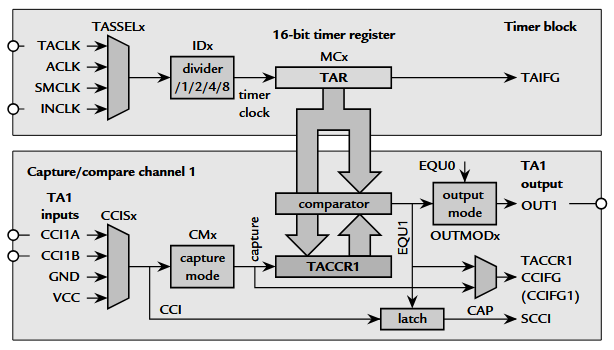
\includegraphics[width=1.0\textwidth]{../Bilder/BlockDiagram_TimerB.png}
	\caption{Timer B Block \& Capture/Compare Channel 1\\\Zitat[S. 355, Kap. 8.16]{davies:msp430}}
	\label{fig:BlockDiagramm_Timer}
\end{figure}

Die Darstellung \Abbildung{BlockDiagramm_Timer} des Timer B als Block Diagram verbildlicht die grundlegenden Komponenten eines Timer-Kanals und deren Zusammenspiel. Die flexiblen Konfigurationsm\"oglichkeiten dieser einzelnen Bl\"ocke erm\"oglichen die Realisierung einer Vielzahl von Zeitsteuerungs- und Signalverarbeitungsaufgaben in eingebetteten Systemen mit dem MSP430FR5729.

\newpage
\subsection{Enhanced Universal Serial Communication Interface (eUSCI)}
\label{eUSCI}


\newpage
\section{Konzeprionierung Observer-Modul}
\label{Grundger\"ust_ObserverModul}


\newpage
\section{Interruptgesteuertes Lesen und Schreiben}
\label{Interruptgesteuertes_Lesen&Schreiben}


\newpage
\section{Debugging-Methoden: Hardware- vs. Software-Breakpoints}
\label{Hardware_VS_Software_Breakpoints}

Im Kontext der Fehlersuche und Programmanalyse in Embedded Systems stellen \Fachbegriff[Bezeichnet in der Softwareentwicklung eine vom Entwickler bewusst gesetzte Unterbrechung im Programmablauf, die typischerweise zur Laufzeit-Debugging-Zwecken verwendet wird. Beim Erreichen dieses Punkts wird die Ausf\"uhrung des Programms angehalten, sodass der aktuelle Zustand (\zB Variableninhalte, Stack, Speicher) analysiert werden kann.]{Breakpoints} ein fundamentales Werkzeug dar. Sie erm\"oglichen es, die Ausf\"uhrung eines Programms an einer vordefinierten Stelle zu unterbrechen, um den internen Zustand des Systems zu inspizieren. Grunds\"atzlich lassen sich zwei prim\"are Arten von Breakpoints unterscheiden: Software-Breakpoints und Hardware-Breakpoints, deren Implementierung und Eigenschaften sich signifikant unterscheiden.

Software-Breakpoints werden zur aktiven Laufzeit des Programms durch einen direkten Eingriff in den ausf\"uhrbaren Code im Speicher des Mikrocontrollers realisiert. An der Zieladresse wird hierbei die urspr\"ungliche Programminstruktion tempor\"ar durch eine Breakpoint-Instruktion oder einen Trap-Befehl ersetzt, der einen Software-Interrupt oder eine Exception ausl\"ost. Sobald der Programmz\"ahler diese modifizierte Stelle erreicht, unterbricht der Mikrocontroller den normalen Programmfluss der Programmzähler stoppt und eine Debug-Routine wird ausgeführt. Der \Fachbegriff[Ein Werkzeug zur schrittweisen Ausf\"uhrung und Analyse von Programmen. Es erlaubt das Setzen von Haltepunkten, das \"uberpr\"ufen von Speicherinhalten und das Nachvollziehen von Kontrollfl\"ussen zur Fehlersuche und -behebung.]{Debugger} kann diesen Zustand erkennen, die urspr\"ungliche Instruktion wiederherstellen und dem Entwickler die Kontrolle \"ubergeben. Durch diesen Mechanismus sind Software-Breakpoints hochflexibel und k\"onnen an nahezu jeder beliebigen Stelle im beschreibbaren Code-Speicher (wie RAM oder FRAM) gesetzt werden.

Die Vorteile des softwarebasierten Ansatzes liegen prim\"ar in der M\"oglichkeit, eine praktisch unbegrenzte Anzahl von Breakpoints im System zu verwenden, sowie in den geringen Anforderungen an zus\"atzliche, dedizierte Hardwarekomponenten auf dem Zielsystem selbst. Die grundlegende F\"ahigkeit, Interrupts oder Exceptions zu behandeln, ist hierf\"ur ausreichend. \Zitat[Kap. 4.7.16]{ti:CCS}

Gegen\"uber den Software-Breakpoints bieten hardwarebasierte Breakpoints den Vorteil, dass sie Programmunterbrechungen auch in solchen Speichersegmenten erm\"oglichen, die schreibgesch\"utzt sind (z.B. ROM oder spezifisch gesch\"utzte Flash-Bereiche). Ein weiterer entscheidender Vorteil ist ihre Nicht-Intrusivit\"at: Da keine Modifikation des Programmcodes stattfindet, werden weder die Konsistenz des Codes im Speicher noch das pr\"azise Echtzeitverhalten (Timing) des Programms durch den Breakpoint-Mechanismus selbst beeinflusst. \Zitat[Kap. 4.7.16]{ti:CCS}, \Zitat[S. 54, Kap. 4.3]{ti:spru296}

Um dies jedoch zu erreichen, ben\"otigen Hardware-Breakpoints ein dediziertes Hardwaremodul innerhalb des Mikrocontrollers. Im Falle der MSP430-Mikrocontrollerfamilie ist dies das \NeuerBegriff{Embedded Emulation Module (EEM)} \Zitat[S. 569, Kap. 21]{ti:slau272d}. Dieses Modul beinhaltet spezielle Hardwareregister, typischerweise Adresskomparatoren, welche die Speicheradresse des Befehls halten, an welcher bei \"ubereinstimmung mit dem Programmz\"ahler ein Breakpoint ausgel\"ost werden soll. Da der Breakpoint durch externe Hardwarelogik ausgel\"ost wird und nicht durch eine im Programmablauf ausgef\"uhrte Instruktion, m\"ussen seitens des Breakpoint-Mechanismus selbst keine Registerinhalte oder Stack-Elemente explizit zwischengespeichert und im Nachhinein wiederhergestellt werden. Ganz im Unterschied wie es bei einem durch einen Software-Breakpoint induzierten Interrupt der Fall sein kann. Die Zustandssicherung erfolgt erst durch die Debug-Routine nach erfolgter Unterbrechung. Der wesentliche Nachteil hierbei ist allerdings die strikte Limitierung der Anzahl gleichzeitig setzbarer Hardware-Breakpoints, welche direkt von der Anzahl der im EEM verf\"ugbaren Komparator-Register abh\"angt. F\"ur den MSP430 sind dies oft nur zwei oder drei \Zitat[vgl. Kap. 7.1]{ti:CCS}.

Diese Gegen\"uberstellung offenbart einen klaren \Fachbegriff[Abwägung zwischen zwei konkurrierenden Zielen, Konzepten, oder ähnlichem, bei der die Verbesserung des einen mit der Verschlechterung des anderen einhergeht.]{Trade-off}: Hardware-Breakpoints gl\"anzen durch ihre Transparenz und die F\"ahigkeit, in gesch\"utzten Speicherbereichen zu operieren, sind jedoch eine knappe Ressource. Software-Breakpoints hingegen bieten eine hohe Flexibilit\"at und nahezu unbegrenzte Verf\"ugbarkeit, gehen aber mit einer leichten Modifikation des Programmcodes und potenziellen, wenn auch meist minimalen, Timing-Ver\"anderungen einher. Angesichts der begrenzten Anzahl an Hardware-Breakpoints auf der MSP430-Plattform, die insbesondere bei komplexeren Debugging-Szenarien schnell ersch\"opft sein k\"onnen, erweist sich die Implementierung von Software-Breakpoints als eine pragmatische und oft notwendige Erweiterung der Debugging-M\"oglichkeiten. Um die technischen Rahmenbedingungen f\"ur die Realisierung solcher Software-Breakpoints auf dem MSP430FR5729 sowie die Interaktion mit der Debugging-Infrastruktur genauer zu verstehen, ist eine detaillierte Betrachtung des eingesetzten Debug-Adapters und seiner Funktionsweise unerl\"asslich. 

Dar\"uber hinaus existiert auch noch eine spezielle Art von Breakpoints welcher von einem Speicherzugriff ausgl\"o{\ss}t wird. Watchpoints k\"onnen Grenzf\"alle identifizieren um dadurch invalide Speicheradressen und zugriffe sowie Puffer\"uberl\"aufe zu analysieren. \Zitat[Kap. 7.4.16.2]{ti:CCS}

Die nachfolgende Analyse des MSP-FET Debuggers wird weitere Aspekte des Software und Hardware-Basierten Debuggings beleuchten und die Grundlage f\"ur die sp\"atere Implementierungsstrategie legen.

\subsection{Der MSP-FET Download Adapter im Detail}
\label{sec:MSP-FET_Debugger}

Die effektive Nutzung von sowohl Hardware- als auch Software-Breakpoints auf dem MSP430FR5729 ist ma{\ss}geblich von der externen Debugging-Hardware und -Software abh\"angig. Als zentrale Schnittstelle zwischen der Entwicklungsumgebung auf dem Host-PC und dem Ziel-Mikrocontroller dient in diesem \"okosystem der \NeuerBegriff{MSP-FET (Flash Emulation Tool) Debugger}. Dieses externe Ger\"at stellt die physische und logische Verbindung zum MSP430 her und erm\"oglicht tiefgreifende Eingriffe und Beobachtungen w\"ahrend der Programmausf\"uhrung.

Der MSP-FET kommuniziert mit dem MSP430-Mikrocontroller typischerweise \"uber standardisierte (Debug-)Schnittstellen wie \NeuerBegriff{JTAG (Joint Test Action Group)} oder das von Texas Instruments entwickelte \Fachbegriff[Zweidraht-Variante des JTAG-Protokolls, die Pin-Anzahl am Target reduziert und besonders f\"ur platzkritische Anwendungen von Vorteil ist.]{Spy-Bi-Wire (SBW)}. \"uber diese Schnittstellen erh\"alt der MSP-FET Zugriff auf das EEM des MSP430FR5729. Wie im vorherigen Abschnitt \ref{Hardware_VS_Software_Breakpoints} dargelegt, ist das EEM f\"ur die Realisierung von Hardware-Breakpoints zust\"andig. Der MSP-FET agiert hierbei als Vermittler, der die vom Entwickler in der \NeuerBegriff{IDE (Integrated Development Environment)} gesetzten Hardware-Breakpoint-Adressen in die entsprechenden Register des EEM schreibt und die vom EEM generierten Haltesignale empf\"angt und an die IDE weiterleitet. Somit ist der MSP-FET unerl\"asslich f\"ur die Konfiguration und Nutzung der limitierten, aber pr\"azisen Hardware-Breakpoint-Ressourcen des Mikrocontrollers. \Zitat[S. 58, Kap. 3.4]{davies:msp430}

Dar\"uber hinaus spielt der MSP-FET eine ebenso gro{\ss}e Rolle f\"ur die Implementierung und Handhabung von Software-Breakpoints. Die F\"ahigkeit, den Speicher des MSP430FR5729 (sowohl RAM als auch das beschreibbare FRAM) zur Laufzeit zu lesen und zu schreiben, ist die Grundvoraussetzung, um Instruktionen mit einer Software-Breakpoint-Routine zu ersetzen. Der Debugger liest \"uber den MSP-FET die urspr\"ungliche Instruktion an der Zieladresse aus, ersetzt diese durch eine Breakpoint-Instruktion und, nach dem Ausl\"osen des Software-Interrupts, stellt er die urspr\"ungliche Instruktion wieder her. Ferner erm\"oglicht der MSP-FET die Steuerung des Programmflusses (Anhalten, Starten, Einzelschrittbetrieb) und den Zugriff auf CPU-Register und Speicherinhalte, was f\"ur die Analyse des Systemzustands an einem Breakpoint unerl\"asslich ist. Das vom Software-Breakpoint ausgel\"oste Interrupt- oder Exception-Signal wird ebenfalls \"uber die Debug-Schnittstelle an den MSP-FET und somit an die Host-Debugger-Software gemeldet.

Es ist wichtig zu verstehen, dass der MSP-FET prim\"ar die Kommunikationsinfrastruktur und die Low-Level-Zugriffsmechanismen bereitstellt. W\"ahrend er das Setzen von Hardware-Breakpoints direkt \"uber das EEM steuert, stellt er f\"ur Software-Breakpoints die notwendigen Lese-, Schreib- und Kontrolloperationen zur Verf\"ugung. Die eigentliche Logik eines Software-Breakpoints – das hei{\ss}t, welche Instruktion als Breakpoint-Befehl dient, wie die urspr\"ungliche Instruktion gesichert und wiederhergestellt wird sowie der resultierende Trap behandelt wird – muss in der Debugger-Software auf dem Host und gegebenenfalls durch eine minimale Debug-Monitor-Routine auf dem Target implementiert werden, wobei der MSP-FET als Br\"ucke dient. \Zitat{ti:slau654e}, \Zitat[S. 56, Kap. 10]{ti:slau157as}

Die Kenntnis der Funktionalit\"aten und der Arbeitsweise des MSP-FET ist somit entscheidend f\"ur die Entwicklung einer robusten Software-Breakpoint-L\"osung. Er definiert die Grenzen und M\"oglichkeiten, wie mit dem Target-System interagiert werden kann, um Breakpoints zu setzen, Zustandsinformationen abzufragen und die Programmausf\"uhrung zu steuern. Die im Folgenden zu entwickelnde Strategie zur Implementierung von Software-Breakpoints muss sich daher eng an den durch den MSP-FET und die Debug-Schnittstelle des MSP430FR5729 gegebenen Rahmenbedingungen orientieren.

\newpage
\subsection{Konzeptionierung von Software-Breakpoints}
\label{sec:KonzeptionierungSoftwareBreakpoints}

Zur Realisierung von Breakpoints existieren mehrere Ans\"atze. Ein bew\"ahrter Einstieg besteht darin, etablierte Debugger und ihre Architektur zu studieren. Im Embedded‑ und Low‑Power‑Bereich kommen beispielsweise Werkzeuge wie \NeuerBegriff{TRACE32}, \NeuerBegriff{M-Core} oder das \NeuerBegriff{MSP-FET} von Texas Instruments zum Einsatz. Diese Debugger setzen Hardware-Breakpoints \"uber spezielle Debug‑Interfaces um und bieten damit eine hohe Zuverl\"assigkeit bei minimaler Eingriffstiefe in das Laufzeitsystem.

Im Gegensatz dazu zielt die hier vorgestellte L\"osung auf eine Abwandlung der Software-Breakpoints ab, die direkt den Programmspeicher manipuliert. Dabei wird, in dieser Implementierung, an der gew\"unschten Halteadresse der originale Maschinenbefehl durch einen Sprungbefehl (Jump) ersetzt, der auf eine speziell implementierte \NeuerBegriff{Breakpoint-Handler}-Routine verweist. Beim Erreichen dieses Befehls wird zun\"achst ein kritischer Abschnitt eingeleitet: Es werden die f\"ur den Prozess relevanten Register – namentlich \Fachbegriff[Ein Register, das die Speicheradresse des derzeitigen Befehls enth\"alt.]{Program Counter (PC)}, \Fachbegriff[Ein Register, das die Speicheradresse des letzten oder ersten Datenelements im Stack speichert.]{Stack Pointer (SP)}, \Fachbegriff[Register f\"ur eine Reihe von Flags, die von der arithmetisch-logischen Einheit in Abh\"angigkeit der zuletzt durchgef\"uhrten Rechenoperation gesetzt werden.]{Statusregister (SR)} und \ggf mehrere \NeuerBegriff{General-Purpose-Register (R4 bis R15)} – gesichert und Interrupts deaktiviert, um eine atomare Kontextsicherung zu gew\"ahrleisten \Zitat[S.91, Kap. 4.3]{ti:slau272d}. Anschlie{\ss}end erfolgt der \"ubergang in die Handler-Routine, die das gesamte System bis auf das Observer-Modul blockiert und so das Auslesen und Manipulieren von Speicherinhalten erm\"oglicht.

Nach der Analyse kann der urspr\"ungliche Programmzustand durch das laden der Registers\"atze wiederhergestellt werden. Eine explizite reaktivierung der Interrupts ist daher nicht n\"otig. Der Compiler stellt hierf\"ur \Fachbegriff[Compiler-spezifische, vordefinierte Funktionen, die direkt in optimierten Assemblercode umgesetzt werden.]{Compiler-Intrinsics} bereit wie \NeuerBegriff{\_\_get\_SR()}, \NeuerBegriff{\_\_get\_SP()} und \NeuerBegriff{\_\_set\_interrupt\_state()} \Zitat[S.137, Kap. 6.8.1]{ti:slau132r}. Auf diese Weise wird ein vollst\"andiger Zyklus von Unterbrechung, Inspektion und Fortsetzung des Programmflusses realisiert, ohne dass das Hauptprogramm von dem Observer-Modul tiefgreifender beeinflusst wird.

Vor diesem Hintergrund wird in den folgenden Abschnitten die Konzeptionierung erweiterter Software-Breakpoints im Detail erl\"autert und auf die daf\"ur notwendigen Voraussetzungen eingegangen.


\subsubsection{Verwendung eines Sprungbefehls anstelle einer Trap}
\label{sec:JumpVsTrap}

Wie in Abschnitt \ref{Hardware_VS_Software_Breakpoints} erl\"autert, basieren klassische software-Breakpoints h\"aufig auf sogenannten Trap-Instruktionen. Das Debugging-Framework der Entwicklungsumgebung unterst\"utzt dies unter anderem \"uber die \NeuerBegriff{General Extension Language} (\Abkuerzung[General Extension Language]{GEL}) – ein Makro- und Skriptsystem, das die Initialisierung von Systemen sowie die Steuerung von Debug-Sitzungen erm\"oglicht. Darüber hinaus erlaubt GEL auch das Setzen von Breakpoints, Speicherzugriffe und die Ablaufkontrolle des Programms \Zitat[Kap. 7.7, 7.7.8.6 \& 7.7.8.7]{ti:CCS}.

Für diese Arbeit war es jedoch erforderlich, dass bei Ausl\"osen eines Breakpoints benutzerdefinierte Routinen aus dem Observer-Modul aktiv bleiben und verwendet werden k\"onnen (\Vgl Abschnitt \ref{Interruptgesteuertes_Lesen&Schreiben}). Diese Funktionalit\"aten sind mit dem Standardverhalten von GEL-Traps nicht kompatibel, da sie typischerweise nur auf Debugger-seitige Prozesse abzielen und keine Kontextintegration benutzerdefinierter Routinen auf dem Zielsystem erlauben.

Aus diesem Grund wurde bewusst auf die Verwendung eines Trap-Mechanismus verzichtet und stattdessen ein direkter Sprungbefehl (Jump) auf eine benutzerdefinierte Breakpoint-Handler-Routine implementiert. Dadurch wird sichergestellt, dass das Observer-Modul auch w\"ahrend einer Unterbrechung aktiv bleibt und die Kontrolle \"uber Register- und Speicherzugriffe erhalten bleibt.


\subsubsection{Implementierung Simpler Software Breakpoints}
\label{sec:ImplementierungSoftwareBreakpoints}

Die Grundidee einfacher Software-Breakpoints besteht darin, an einer Stelle im Programmspeicher, an der ein g\"ultiger Maschinenbefehl (\Fachbegriff[Auch op code oder operation code, ist eine meist in hexadezimaler Schreibweise angegebene Zahl, die die Nummer eines Maschinenbefehls f\"ur einen bestimmten Prozessortyp angibt.]{Opcode}) liegt, diesen tempor\"ar durch einen Sprung auf die Breakpoint-Handler-Routine zu ersetzen. Zun\"achst wird der originale Opcode gesichert, um ihn sp\"ater unver\"andert wieder einsetzen zu k\"onnen. Die Auswahl der Adresse erfordert, dass diese auf ein g\"ultiges Befehlswort ausgerichtet ist und im Stack-Bereich liegt, um Kollisionen auf das Code-Segmenten zu vermeiden.

Die Implementierung gliedert sich in folgende Schritte:
\begin{enumerate}
\item \textbf{Adressvalidierung:} Pr\"ufen, ob die Zieladresse auf ein Doppelwort (8 Bytes) ausgerichtet ist und im Stack liegt.  
\item \textbf{Kontext-Sicherung:} In einem kritischen Abschnitt werden PC, SP, SR und alle modifizierten Register in einem Puffer abgelegt.  
\item \textbf{Ersetzen des Opcodes:} Der Original-Opcode (8 Bytes) wird durch den 8-Byte-Sprungbefehl (4 Bytes f\"ur den Instruction-Code, 4 Bytes f\"ur die Zieladresse der Handler-Routine) \"uberschrieben. \Zitat[S.161, Kap. 4.6.2.28]{ti:slau272d}
\item \textbf{Ausf\"uhrung des Breakpoint-Handlers:} Beim Eintreten des Breakpoint-Opcodes springt der PC in die Handler-Routine, die das System an weiterer Ausf\"uhrung hindert und stattdessen das Observer-Modul f\"ur weitere Debug-Schritte aktiv h\"alt.
\item \textbf{Kontext-Wiederherstellung:} Nach Abschluss der Debug-Aktion werden alle Register und der urspr\"ungliche Opcode wiederhergestellt, bevor der normale Programmablauf fortgesetzt wird.
\end{enumerate}

Diese Vorgehensweise stellt die R\"uckkehr zum urspr\"unglichen Systemzustand – einschlie{\ss}lich des Originalen-Opcodes – sicher und garantiert die Konsistenz des Programms.

Um die im vorigen Abschnitt \ref{sec:KonzeptionierungSoftwareBreakpoints} skizzierten Konzepte robust umzusetzen, sind die im n\"achsten Abschnitt, technischen Details wie Instruktionsl\"angen und Speicher-Alignment, zu betrachten.

\subsubsection{Instruktionsl\"angen und Speicher-Alignment}
\label{sec:TechnischeUmsetzunSoftwareBreakpoints}

Die Manipulation von Befehlen im Stack ist hoch kritisch, da das Hauptprogramm keine Kenntnis vom Observer-Modul hat und eine falsche Adressierung oder unvollst\"andige Opcode-substituierung zu undefiniertem Verhalten f\"uhren kann. Zwei zentrale Aspekte sind dabei zu beachten:

\begin{itemize}
	\item \textbf{Speicher-Alignment:} MSP430-Instruktionen sind grundsätzlich an geraden Speicheradressen ausgerichtet. Vor jedem Schreib- oder Lesezugriff muss daher sichergestellt werden, dass die Zieladresse eine gerade Adresse ist. Zugriffe auf ungerade Adressen können zu undefiniertem Verhalten führen, sofern keine Fehlerbehandlung erfolgt. Darüber hinaus sind Adressen, die in der Mitte eines Opcodes liegen, ungültig und dürfen nicht als Breakpoint oder adressiert werden.
	\item \textbf{Opcode-L\"angen:} W\"ahrend einzelne Maschinenbefehle in der Regel vier bis acht Bytes belegen, k\"onnen komplexe Instruktionen – etwa \texttt{MOV.\allowbreak W} – bis zu zwölf Bytes lang sein \Zitat[S.165, Kap. 4.6.2.32]{ti:slau272d}. Diese Variabilit\"at erschwert das gezielte \"Uberschreiben von genau acht Bytes, die f\"ur die Jump-Instruktion einschlie{\ss}lich Zieladresse ben\"otigt werden. Unter diesen Randbedingungen besteht die Gefahr, dass entweder zu viele oder zu wenige Bytes \"uberschrieben werden, was zu ung\"ultigen oder unbeabsichtigten Instruktionen f\"uhren kann.
\end{itemize}

Das Sichern und Wiederherstellen von Registern und des Originalen Opcodes reicht daher nicht aus. Es wird eine Kopie des Stacks ben\"otigt, in welcher der bestehende Opcode Manipuliert wird. Dies garantiert ein sicheres zur\"uckkehren in die Hauptroutinen, sowie eine Robuste Ausf\"uhrung der Funktion zum verarbeiten der \ggf mehreren Breakpoints.

Dies erschwert die Umsetzung und erh\"oht die Komplexit\"at der Routine erheblich, wodurch Timing und Konsistenz gef\"ahrdet werden. Im anschlie{\ss}enden Fazit werden die gewonnenen Erkenntnisse bewertet, offene Fragestellungen skizziert und ein Ausblick auf weiterf\"uhrende Arbeiten gegeben.

\subsection{Fazit zur Umsetzung von Software Breakpoints}
\label{sec:FazitSoftwareBreakpoints}

Die Realisierung von Software-Breakpoints auf dem Low‑Power‑Mikrocontroller MSP430FR5729 erfordert ein tiefgehendes Verst\"andnis der Prozessor‑Architektur, der Instruktionsformate und der nebenl\"aufigen Abl\"aufe im System. Die Analyse der Problemstellung hat ergeben, dass unter anderem kritische Bereiche atomar bearbeitet, Register und Stack-Zust\"ande zuverl\"assig gesichert und Intrinsics korrekt eingesetzt werden m\"ussen. Zudem sind umfangreiche Funktionen zur \"uberwachung und Protokollierung des Systemzustands zu implementieren.

Die erwartete komplexit\"at inklusive der Anforderungen an Robustheit, Echtzeitf\"ahigkeit und m\"oglichst geringem Eingriff in den Betrieb \"uberschreitet den Rahmen einer \"ublichen Bachelorarbeit. Eine vollst\"andige, ausgereifte Implementierung w\"are mit dem Umfang einer Masterarbeit oder vergleichbarer Forschungsarbeiten m\"oglich. Dennoch bildet dieses Thema eine exzellente Grundlage f\"ur weiterf\"uhrende Arbeiten in den Bereichen eingebettete Echtzeitsysteme und Debugging‑Technologien.

